%%%%%%%%%%%%%%%%%%%%%%%%%%%%%% BEGIN EXECUTION_MODEL.tex %%%%%%%%%%%%%%%%%%%%%%%

What could we do with such a representation? It is important to understand why we don’t work with some intermediate representation like bytecodes. By working in the target programming language, we can take advantage of both the abstractions afforded by the language and the expert knowledge of the programmer about how to exploit those abstractions. The apprentice is bootstrapped with several statistical language models: one trained on a natural language corpus and the other on a large code repository. Using these resources and the means of representing and manipulating program embeddings, we intend to train the apprentice to predict the next expression in a partially constructed program by using a variant of imagination-based planning~\cite{PascanuetalCoRR-17}. As another example, we will attempt to leverage NLP methods to generate proposals for substituting one program fragment for another as the basis for code completion. 

%%% %%%%%%%%%%%%%%%%%%%%%%%%%%%%%%%%%%%%%%%%%%%%%%%%%%%%%%%%%%%%%%%%%%%%%%%%%%%%

%%% Figure~{\urlh{#fig_Differentiable_Program_Emulation}{\ref{fig_emulator}}}
\begin{figure}
%
  \begin{center} 
%    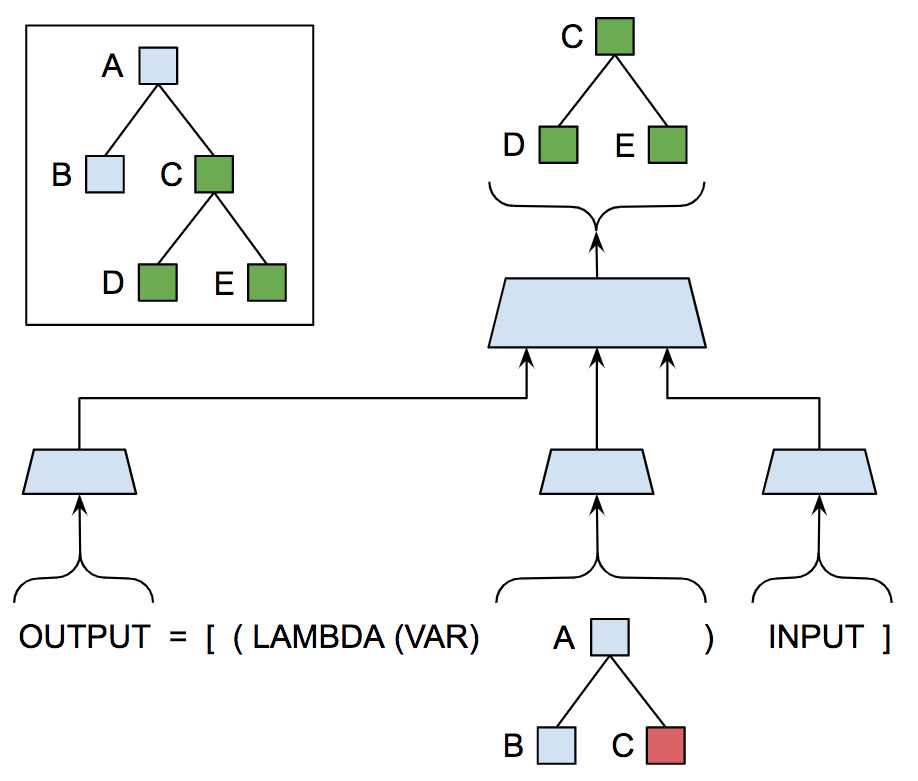
\includegraphics[width=5.3125in]{./figures/Differentiable_Program_Emulation.png} % 918 × 781 pixels
    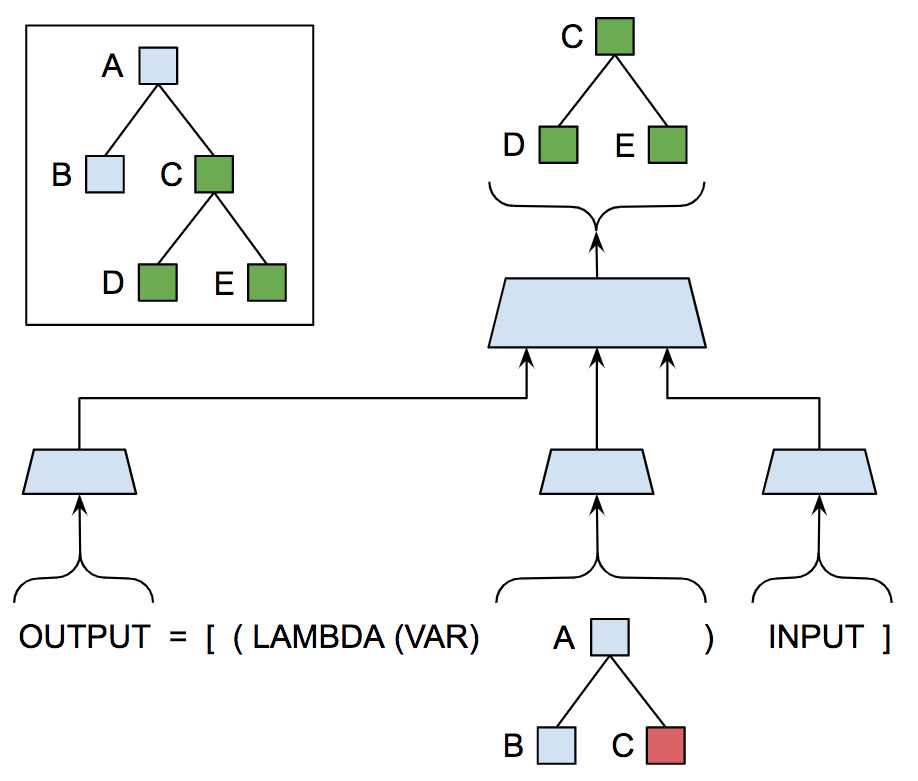
\includegraphics[width=2.65in]{./figures/Differentiable_Program_Emulation.png} % 918 × 781 pixels
  \end{center}
%
  \caption{This slide illustrates how we make use of input / output pairs as program invariants to narrow search for the next statement in the evolving target program. At any given moment the call stack contains the trace of a single conditioned path through the developing program. A single path is unlikely to provide sufficient information to account for the constraints implicit in all of the sample input / output pairs and so we intend to use a limited lookahead planning system to sample multiple execution traces in order to inform the prediction of the next program statement. 
%
These so-called imagination-augmented agents implement a novel architecture for reinforcement learning that balances exploration and exploitation using imperfect models to generate trajectories from some initial state using actions sampled from a rollout policy~\cite{PascanuetalCoRR-17,WeberetalCoRR-17,HamricketalCoRR-17,GuezetalCoRR-18}. These trajectories are then combined and fed to an output policy along with the action proposed by a model-free policy to make better decisions. There are related reinforcement learning architectures that perform Monte Carlo Markov chain search to apply and collect the constraints from multiple input / output pairs.}
%
  \label{fig_emulator}
%
\end{figure}

%%% %%%%%%%%%%%%%%%%%%%%%%%%%%%%%%%%%%%%%%%%%%%%%%%%%%%%%%%%%%%%%%%%%%%%%%%%%%%%

The Differentiable Neural Program (DNP) representation and associated NTM controller for managing the call stack and single-stepping through such programs allow us to exploit the advantages of distributed vector representations to predict the next statement in a program under construction. This model makes it easy to take advantage of supplied natural language descriptions and example input / output pairs plus incorporate semantic information in the form of execution traces generated by utilizing the FIDE to evaluate each statement and encoding information about local variables on the stack.

%%%%%%%%%%%%%%%%%%%%%%%%%%%%%% END EXECUTION_MODEL.tex  %%%%%%%%%%%%%%%%%%%%%%%%
